%%% ---------------------------------------------------------------------------------
%%% Vorlage Abschlussarbeit (LaTeX)
%%% 
%%% V1   03/2017, Stefan Etschberger (HSA)
%%% V1.1 04/2021, rnw-hack für biblatex-run
%%% V2   05/2021, Titelblatt und Erweiterungen: Stefan Jansen (HSA)
%%% V2.1 05/2021, Trennung von R-Support und einfachem LaTeX: Phillip Heidegger (HSA)
%%% V2.2 01/2024, Anpassung an THA-Layout
%%% V3   01/2024, I18n
%%% V3.1 10/2024, Phillip Heideger, Online Version präferiert, Reparatur langes Inhaltsverzeichnis,
%%%               Erklärung Referenzen, blau für Refs & Links
%%% ---------------------------------------------------------------------------------
\documentclass[12pt,a4paper%
              ,oneside     % fuer PDF-Abgabe, bei Druck twoside
              ,titlepage
              ,DIV=13
              ,headinclude
              ,footinclude=false%
              ,cleardoublepage=empty%
              ,parskip=half,
              BCOR=0mm,
              ]{scrreprt}

\usepackage[utf8]{inputenc}
\usepackage[T1]{fontenc}

\usepackage[authorName={Andreas Alstetter}
           ,authorEnrolmentNo={2147455}
           ,authorStreet={Pfarrer-Kempter Str.~4}
           ,authorZip={89358}
           ,authorCity={Kammeltal/Behlingen}
           ,authorEMail={andreas.alstetter@tha.de}
           ,authorPhone= {+49\,3141-5926}
           ,authorSignaturePlace={Augsburg}
           ,studyProgram={Mathematik}
%           ,thesisType={Bachelorarbeit}
           ,thesisTitle={Proximitätssuche von EPLAN-Makros auf Basis des LambdaRank-Algorithmus}
           ,studyDegree=%
%                        {{Bachelor of Arts}}
                        {{Bachelor of Engineering}}
%                        {{Bachelor of Science (B.\,Sc.)}}
%                        {{Master of Arts}}
%                        {{Master of Engeneering}}
%                        {{Master of Science (M.\,Sc.)}}
           ,faculty=% 
%                     {{Fakultät für \\ Angewandte \\ Geistes-  und  \\ Naturwissenschaften}}
%                     {{Fakultät für \\ Architektur und \\ Bauwesen}}
%                     {{Fakultät für \\ Elektrotechnik}}
%                     {{Fakultät für \\ Gestaltung}}
                     {{Fakultät für \\ Informatik}}
%                     {{Fakultät für \\ Maschinenbau und \\ Verfahrenstechnik}}, showDiesel=true
%                     {{Fakultät für \\ Wirtschaft}}
%           ,topicAssignment={\today}
%           ,submissionDate={\today}
%           ,defenseDate={\today}
%           ,nonDisclosure={false}
           ,supervisor={Prof.~Dr.~Thomas Kirchmeier}
           ,supervisorDeputy={Prof.~Dr.~Jürgen Grinninger}
%           ,language={en}
           ]{THA-Abschlussarbeit}

% ====== mögliches Setup fürs PDFs =======
\hypersetup{
  colorlinks=true,
  allcolors = THAi-Blue, % oder THAred ??
  linktocpage  
}
% Siehe:
% https://ctan.net/macros/latex/contrib/hyperref/doc/hyperref-doc.pdf
% S. Kap. 5, S. 10 ff

% Ohne diese Zeile: Mit klickbaren links
% \hypersetup{draft}


% Literaturdatenbank (.bib-Datei) aus Citavi o.ä.
\bibliography{Literatur_Abschlussarbeit}

\graphicspath{{Bilder/}}

\usepackage{caption}
\DeclareCaptionLabelFormat{something}{#2.#1.}
\captionsetup[lstlisting]{labelformat=something}

\begin{document}

% Sprachauswahl zum Umschalten innerhalb des Textes. 
% Alternativen: \thesisLanguage, ngerman, english
\selectlanguage{\thesisLanguage}

\pagenumbering{roman}
\setcounter{page}{1}

\THAtitlepage

\tableofcontents

%%% --------------------------------------------------
%%% Ab hier: Inhalt
%%% --------------------------------------------------

\setcounter{page}{1}
\pagenumbering{arabic}


\begin{figure}
\centering
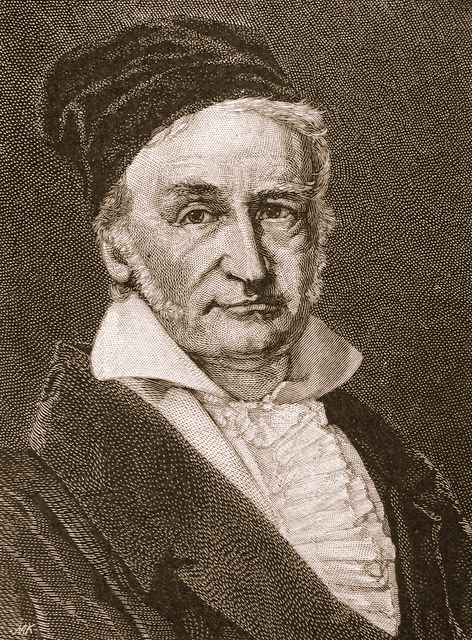
\includegraphics[ angle=0, width=.3\textwidth]{karl_friedrich_gauss}
\caption{\index{Grafik}\index{jpg}Ein jpeg-Bild, hier mit Gauß darauf\label{fig:Gauss}}\par
\end{figure}



% -----------------------------------------------------
\section{Einträge im Stichwortverzeichnis}

Einträge im Stichwortverzeichnis können über den \lstI{index}-Befehl generiert werden. Zum Beispiel soll der Begriff \emph{Bachelorarbeit}\index{Bachelorarbeit} hier referenziert werden. Außerdem sollen noch die Begriffe Apfel\index{Apfel}, Birne\index{Birne} und Zebra\index{Zebra} ins Verzeichnis. Damit unter dem Buchstaben mehr als ein Eintrag steht, nehmen wir noch \emph{Buch}\index{Buch} und Brille\index{Brille} auf. 

\chapter{Motivation}
Die zunehmende Digitalisierung von industriellen Prozessen führt zu einer immer größer werdenden Menge an Prozess- und Produktdaten.
Die Informationen liegen dabei oft in strukturierter und unstrukturierter Form wie Datenblätter, Produktbeschreibungen sowie Spezifikationen vor.
Im gleichen Zuge steigt die Bedeutung von datengetriebenen Methoden für die Innovations- und Wettbewerbsfähigkeit in Deutschland. 
KI und dessen Potential die Daten sowie das Know-How der Industrie 4.0 zu nutzen, schafft somit den Grundstein um diese Herausforderung für die Industrie und deren Systeme zu meistern. \cite{Bundesregierung2026}.


Im Anlagen- sowie Maschinenbau entsteht durch die Variantenvielfalt technischer Komponenten eine besondere Herausforderung.
Dabei werden von Unternehmen einerseits häufig umfangreiche Artikelbestände verwaltet, die eine Vielzahl an technischen Merkmalen beinhalten,
während andernseits große Mengen an Dokumentationen und Datenblättern vorliegen.
Eine Auswahl geeigneter Komponenten sowie die Artikelzuordnung zu standardisierten Lösungen erfolgt oftmals auf Basis von manueller Recherche und Erfahrung einzelner Mitarbeiter.
Dadurch entsteht ein hoher Bearbeitungsaufwand, geringere Skalierbarkeit und eine hohen Abhängigkeit von Expertenwissen. \cite{Pfenning2022}.


Arbeiten aus der Wissenschaft zeigen, dass zur erfolgreichen Wissensextraktion, Automatisierung und Entscheidungsfindung KI-Verfahren in industirellen Prozessen eingesetzt werden.
Einer der zentralen Punkte ist dabei die Extraktion von Informationen und Wissen aus aus heterogenen Datenquellen sowie die anschließende Nutzung dieser Extraktion für die technische Entscheidungsfindung.
Als bewährter Ansatz hierfür eignen sich Empfehlungssysteme, die den Anwender dabei unterstützen, die am besten geeigneten Optionen für einen konkreten Anwendugsfall aus einer Vielzahl an Alternativen zu finden.
Die Urspüngliche Verwendung solcher Systeme aus dem E-Commerce-Bereich, werden zunehmend auch im Industriellen Kontext angewendet, wie zum Beispiel bei der Auswahl von Produkten, Konfigurationen oder der erneuten Verwendung von Systemen. \cite{Joshi2024}.

Auf Basis dieser Recherche ergibt sich ein erhebliches Potential für ein KI-basiertes Empfehlungssystem zur automatisierten Zuordnung von EPLAN-Artikeln \cite{EPLANArtikelverwaltung} zu EPLAN-Fenstermakros. \cite{EPLAN2025}.
Hierfür notwendige Informationen sind bereits in den vorhandenen EPLAN-Artikeln \cite{EPLANArtikelverwaltung} sowie den zugehörigen Datenblättern enthalten, werden aber für die automatisierte Verarbeitung bislang nur unzureichend genutzt. 
Die intelligente Auswertung dieser strukturierten und unstrukturierten Daten bietet die Grundlage für die Erkennung relevanter Zusammenhänge und die Empfehlung passendender EPLAN-Fenstermakros. \cite{EPLAN2025}.
Hierdurch wird der manuelle Aufwand entscheidend reduziert, sowie das vorhandene Unternehmenswissen besser genutzt und für eine konsistentere Entscheidungsfindung verwendet.
Das Projekt leiste somit einen Beitrag zur praktischen Umsetzung von datengetriebenen und KI-Unterstützen Entscheidungen im Industrie 4.0 Umfeld. \cite{Nayak2025}.

\chapter{Stand der Technik}

\chapter{Zielsetzung und Vorgehensweise}

\chapter{Analyse der Makrostrukturen und Ableitung eines Trainingsformats}

\chapter{Prototypische Umsetzung}

\chapter{Evaluierungskonzept und Ergebnisse}

\chapter{Diskussion, Grenzen und Ausblick}

\chapter{Zusammenfassung und Fazit}

\appendix

% Selbständigkeitserklärung
\AuthorDeclaration


\listoffigures % Abbildungsverzeichnis
\listoftables % Tabellenverzeichnis

% --------------------------------------------------
% Bibliographie
% --------------------------------------------------
\renewcommand{\bibfont}{\footnotesize}
\printbibliography[title={Literaturverzeichnis}, 
                   heading=bibintoc]


% --------------------------------------------------
% Index
% --------------------------------------------------
{\setkomafont{section}{\Huge} % temporarily set chapter font
\printindex
}

\end{document}
